\documentclass{article}

% Camera-ready: [dblblindworkshop, final] shows the author block and removes line numbers.
\usepackage[dblblindworkshop, final]{neurips_2026}

\workshoptitle{Workshop for Autonomous ML Research}

\usepackage[utf8]{inputenc}
\usepackage[T1]{fontenc}
\usepackage{hyperref}
\usepackage{url}
\usepackage{booktabs}
\usepackage{amsfonts}
\usepackage{amssymb}
\usepackage{amsmath}
\usepackage{nicefrac}
\usepackage{microtype}
\usepackage{xcolor}
\usepackage{graphicx}
\usepackage{enumitem}
\usepackage{array}
\setlist{nosep, leftmargin=1.4em}

\title{Born, Not Trained: Zero-Training Programs\\Out-Explore Reinforcement Learning\\for Game Testing at Equal Budget}

\author{%
  Andy Ye \\
  Paul G. Allen School of Computer Science \& Engineering \\
  University of Washington \\
  \texttt{andy132@cs.washington.edu} \\
}

\begin{document}

\maketitle

\begin{abstract}
Play-testing for new video games is a crucial aspect of game development, as it is important to ensure that nothing breaks when the game goes live. Automated testers do this by exploring the game, and the standard method to build one is to train a reinforcement-learning (RL) agent separately for each game. We ask whether an LLM can instead write the tester once, as a short program that needs no training, and if it can be reused on new games. We started from a simple, well-known exploration program (Go-Explore) and let two Claude models improve it over $36$ rounds, keeping the versions that explored a set of practice games fastest. The whole search cost about \$20 in API calls. We then ran the best program, unchanged, on four games it had never seen: two grid mazes, Breakout, and Sokoban. Every method was allowed the same number of game steps. The program reached $91\%$ ($95\%$ interval $83$ to $98$) of the targets we set, such as winning a level, compared with $54\%$ for a tuned RL agent (PPO), $51\%$ for random play, and $34\%$ for the Go-Explore program we started from. PPO needed $4$ to $16$ times as many game steps to catch up. However, our result has limitations. All of our games are small and two-dimensional. On two easier games our program only ties a trivial baseline, and on Craftax it ties with PPO. We tested actual bug finding on only one physics game, with bugs we planted ourselves, and the gain there was smaller. That test also exposed a bug in our own evaluation code that had made an early result look better than it was, after an LLM code review had passed it.
\end{abstract}

\noindent\textbf{Keywords:} Autonomous ML research; Evolutionary search; Exploration; Game development; Game testing; LLM-driven program synthesis; Reinforcement learning

% ############################################################################
% ####  PART 1  ####  Agent-written research result
% ############################################################################
\section{Autonomous Research Result}
\subsection{Introduction}
\label{sec:intro}
Before a game ships, it is important to check that every level can be finished and that nothing breaks along the way. An automated tester does this by exploring: it plays the game and tries to get into the situations a developer needs to
see, such as the end of a level, a room that is hard to reach, or the exact setup that triggers a bug. It has to do
this within the limited number of game steps a test run can afford. The standard way to build such a tester is to train a
reinforcement-learning (RL) agent with a reward for visiting new states~\citep{tang2017,rnd,icm}. This works, but the
agent has to be trained and tuned again for every game, and training itself uses up many game steps.

We propose a different method. Instead of training a tester, we have an LLM write one as a short program, and we improve
that program over many rounds with an evolutionary search, in the style of FunSearch~\citep{funsearch}. The program is
not trained. It plays many copies of the game at once, saves interesting game states as it goes, and keeps returning to
the most promising ones to explore further. We run the search once, on one set of games, and then reuse the resulting
program on unseen games.

A tester can only find a bug if it first gets the game into the situation where the bug appears, and reaching such situations is the hard part of testing. We therefore compare testers by how well they explore. Each tester gets the same number of game steps, and we count how many \emph{targets} it reaches. A target is a situation we want the tester to bring about, such as reaching the exit of a maze, clearing eight bricks, or pushing two boxes into place. We also check bug finding directly, on a physics game where we planted over 300 bugs (Section~\ref{sec:kinetix}).

Our main result is that our evolved program explores much better than a trained agent when both get the same number of
steps. On four games that it never saw during the search, it reaches $91\%$ of the targets. A tuned PPO agent reaches
$54\%$, and Go-Explore, the base program that the search started from, reaches $34\%$ (Fig.~\ref{fig:main}A). The advantage
disappears if PPO is given $4$ to $16$ times as many steps (Fig.~\ref{fig:main}B), and it is absent on three other
games. On the planted bugs the gain is smaller. Section~\ref{sec:roles} lists which parts of this work were done by the
search, by the AI agent that ran the project, and by us.

\subsection{Problem Setup}
\label{sec:setup}
A tester is a program that controls many copies of a game level at the same time. We call each copy a worker. The
tester also has a fixed number of slots in which it can save game states. At every step it makes three decisions for
each worker: whether to go back to a saved state (\texttt{restore}), which action to take next (\texttt{act}), and
whether to save the worker's current state (\texttt{archive}). Saving and going back is what makes such a tester
efficient. The interesting places in a game are usually many steps from the start, and a tester that always starts over
spends most of its steps getting back to where it already was. A tester that saved a state there can return to it
directly and spend its steps on what lies beyond. To make its decisions the tester sees a short list of numbers that
describe each worker's state: position, velocity, one number for progress, the time elapsed, and a few values specific
to the game (Appendix~\ref{app:protocol}). It is never told what the target is.

Each target is a level together with a condition, for example ``the player is standing on the exit''
(Table~\ref{tab:protocol}). A tester reaches a target if any of its workers meets the condition before the steps run
out. We repeat every run with several random seeds and report the fraction of (target, seed) pairs reached.

Every method gets the same number of game steps per target, $131{,}072$. A tester spends them as $64$ workers playing
$2048$ steps each, and reloading a saved state is free. PPO spends them on training, and we count a target as reached if
PPO reaches it at any point while it trains.

One difference between the methods should be kept in mind. Testers can save and reload game states, and PPO cannot. This
is realistic for a developer who owns the game, but it means we are comparing two different kinds of method. To check how much of the result comes from saving and reloading alone, we include a simple, generic version of Go-Explore~\citep{goexplore}. It saves and reloads states through the same interface, uses one fixed rule on every game, and is the base program of our search.

\subsection{Method}
\label{sec:method}
\begin{figure}[t]\centering
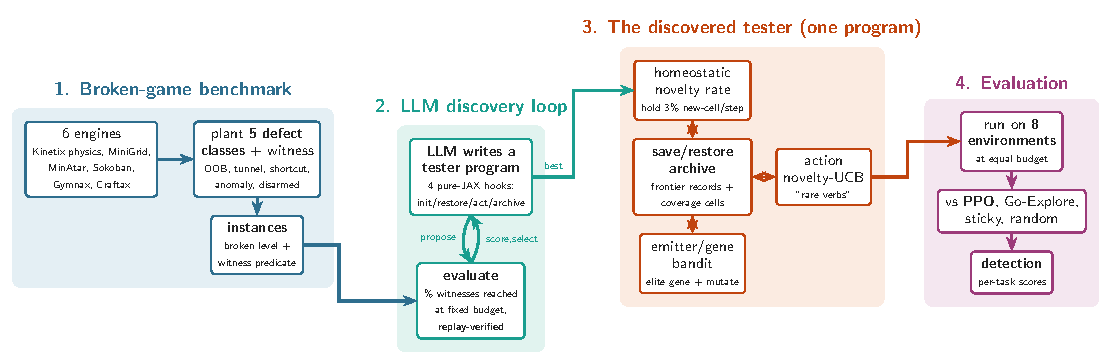
\includegraphics[width=\linewidth]{figs/pipeline.pdf}
\caption{\textbf{Method overview.} (1) The search starts from Go-Explore. An LLM improves the program, each new version
is scored on how quickly it reaches targets, and the best one is kept. (2) The best program makes three decisions at
every step. (3) We run it, unchanged, on four games it has never seen.}
\label{fig:pipeline}
\end{figure}

The search uses ShinkaEvolve~\citep{shinkaevolve} (Fig.~\ref{fig:pipeline}, left). In each round, Claude Sonnet~5 or
Claude Opus~5 is shown an existing program, a few other programs for inspiration, and their scores, and it writes a
modified program, which is then scored. The base program is plain Go-Explore, which saves one state for each region of
the game it has visited, sometimes reloads one of them, and otherwise takes random actions. A program's score rewards reaching targets in fewer steps. For each target it is the share of the step limit that was left when the target was first reached, so it is $0$ if the target is never reached. The score is the average over the targets of a set of practice games. These targets are planted bugs in the physics game Kinetix, achievements in Craftax, and goals in three small control tasks (Appendix~\ref{app:search}). The search scored $36$ programs, and the best score rose from $0.405$ to $0.589$
(Fig.~\ref{fig:evo}). We took the program with the best score and did not edit it afterwards.

The best program is $280$ lines of code (Appendix~\ref{app:program} gives pseudocode), and Fig.~\ref{fig:pipeline}
(middle) summarises how it explores. It differs from Go-Explore in four ways. First, it saves two kinds of state. Like
Go-Explore, it saves a state whenever a worker arrives somewhere new. It also saves record-setting states, meaning the
state with the highest or lowest value seen so far for each number in the state description. A record is often the
furthest the tester has got in some direction, which makes it a good place to continue from. Second, it has six simple
ways of acting where Go-Explore has one, for example random actions, holding one action, or cycling through all
actions. Different games reward different kinds of movement, so the program keeps track of which ways of acting have
recently led to new states and uses those more often, without ever dropping any of them. Third, it works out while it runs which numbers in the
state description behave like progress, meaning that they almost only go up or that they change rarely. Whether a key
is being carried and how many boxes are in place are examples. This tells the program which saved states are worth
going back to, and it prefers the ones that are further along. Fourth, a worker goes back to a saved state whenever it
has been stuck for $40$ steps, and otherwise with a small chance at every step. The program also rescales every number to
the same range, which lets one set of constants work on different games.

Each of these ideas builds on earlier work. Go-Explore~\citep{goexplore} introduced saving and revisiting states, but it
relies on a person to decide for each game which states count as different, and it takes random actions after
returning. Our program makes both choices itself while it runs. RL agents with novelty
rewards~\citep{tang2017,rnd,icm} explore well but have to be trained for each game, and LLM agents that test a game by
playing it step by step~\citep{titan} need the LLM throughout testing. LLMs have also been used to evolve programs
against a score~\citep{funsearch,shinkaevolve}, to write reward functions for RL~\citep{eureka}, and to act as the
policy optimiser~\citep{promptpo}. Our work combines these lines: we evolve an exploration program with an LLM, and we
show that the result works on games it was never evolved on, with no training and no LLM at test time.

\subsection{Experimental Setup}
\label{sec:protocol}
\begin{table}[t]\centering\small
\caption{\textbf{Evaluation games.} Every method gets $131{,}072$ game steps per target ($65{,}536$ on Craftax).}
\label{tab:protocol}
\setlength{\tabcolsep}{5pt}
\begin{tabular}{@{}llcl@{}}\toprule
Game & A target is reached when & Targets & Seen in the search? \\ \midrule
DoorKey (MiniGrid) & the player reaches the exit, which needs a key & $6$ & no \\
FourRooms (MiniGrid) & the player reaches the exit & $6$ & no \\
Breakout (MinAtar) & $3$, $8$, or $15$ bricks are cleared, on $6$ levels & $18$ & no \\
Sokoban (Jumanji) & $1$, $2$, or $3$ boxes are in place, on $6$ levels & $18$ & no \\ \midrule
MountainCar & the car reaches the flag & $6$ & yes \\
DeepSea & the player reaches the treasure & $6$ & a smaller version \\
Craftax & an achievement is unlocked & $32$ & yes \\ \bottomrule
\end{tabular}
\end{table}

We evaluate on seven games (Table~\ref{tab:protocol}). Four unseen games are our main test: DoorKey, FourRooms, Breakout, and Sokoban. These games are hard enough that simple strategies do not reach every target. The other three were used in the search in some form, so we report them separately.

We compare the evolved program against four other methods. Two are simple. Random play picks a random action at every step, and action-repeat picks a random action and holds it for $1$ to $12$ steps~\citep{machado2018}. The third is Go-Explore, the base program of our search, with no tuning. The fourth is PPO, which sees the same state description as the testers. PPO's results depend heavily on its reward and settings, so we trained ten versions of it: five rewards (three novelty rewards from prior work~\citep{tang2017,rnd,icm}, one of our own, and the game's own reward), each with two hyperparameter settings (Appendix~\ref{app:protocol}). For each game we report the best of the ten. We chose it using the same runs that we report, which favours PPO. Testers and the reported PPO versions use five seeds; PPO with more steps uses three seeds and three of the rewards.

\subsection{Results}
\label{sec:result}
\begin{figure}[t]\centering
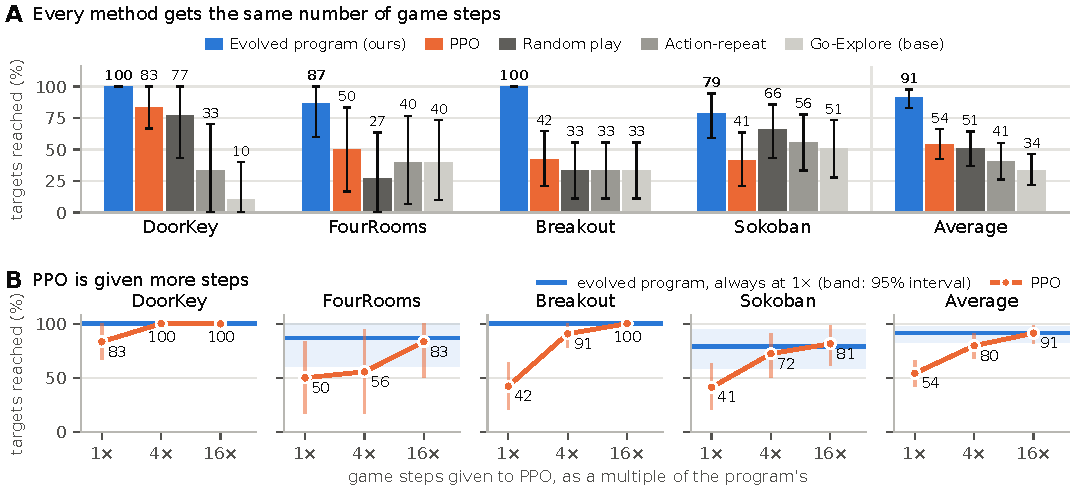
\includegraphics[width=\linewidth]{figs/fig_results.pdf}
\caption{\textbf{Main results on the four unseen games, and their average.} \textbf{(A)} Share of targets reached when
every method gets the same number of game steps. Error bars are $95\%$ bootstrap intervals over levels and seeds. \textbf{(B)} PPO is given $4$ and $16$ times as many steps, while the evolved program stays at
$1\times$ (blue line; the shaded band is its interval).}
\label{fig:main}
\end{figure}

With the same number of steps, the evolved program reaches more targets than every baseline on all four games
(Fig.~\ref{fig:main}A). It reaches $100\%$ on DoorKey, $87\%$ on FourRooms, $100\%$ on Breakout, and $79\%$ on Sokoban,
which averages to $91\%$ ($95\%$ interval $83$ to $98$). PPO reaches $83\%$, $50\%$, $42\%$, and $41\%$, which averages
to $54\%$ ($42$ to $66$). The gap to PPO is $17$ points on DoorKey, $37$ on FourRooms, $58$ on Breakout, and $38$ on
Sokoban, and in each case the interval for the gap excludes zero. Of the $48$ targets, the program does better than PPO
on $32$, the same on $16$, and worse on none (per-seed results are in Appendix~\ref{app:perseed}).

Saving and reloading states does not explain this result by itself. Go-Explore saves and reloads states too, and it
reaches only $34\%$, which is less than random play ($51\%$). The search is what made the difference, taking a program
that reaches $34\%$ on these games and turning it into one that reaches $91\%$, even though it never saw these games. We also tried evolving a program directly on one of the test games. A second, shorter search ($18$ rounds), scored only on DoorKey, produced a program that reaches $33\%$ of the DoorKey targets, far below the $100\%$ reached by the program that was evolved on other games and had never seen DoorKey. In this one comparison, evolving on a mix of games and reusing the result worked better than evolving on the test game itself.

PPO does catch up if it is given more steps (Fig.~\ref{fig:main}B). With $4$ times as many steps its average rises to
$80\%$, and with $16$ times as many it reaches $91\%$, the same as the program. It matches the program on DoorKey at
$4$ times the steps and on Breakout at $16$ times. On FourRooms and Sokoban the two are too close to separate at $16$
times.

The evolved program is not always the better choice. On MountainCar and DeepSea it reaches every target, but so does a trivial method like action-repeat, so games this simple do not need it. On Craftax, which was one of the practice games, the program, PPO, and random play all reach about a third of the targets ($33\%$, $32\%$, and $31\%$), so the program has no advantage there either. We also checked a few extra levels of each main game that we had set aside and did not look at when choosing which program to report (Appendix~\ref{app:perseed}). On those levels the program is again the best on Breakout and Sokoban and ties random play on DoorKey, but on FourRooms it reaches $20\%$ against $50\%$ for action-repeat (on two levels).

\subsection{Bug Finding on Kinetix}
\label{sec:kinetix}
\begin{table}[t]\centering\small
\caption{\textbf{Planted bugs found in Kinetix (\%).} Averages over five seeds, with $262{,}144$ game steps per bug. Every
detection was confirmed by re-running it from the start of the level.}
\label{tab:kinetix}
\begin{tabular}{@{}lccc@{}}\toprule
Tester & Levels used in the search & New levels & New type of bug \\ \midrule
Random play & $49$ & $56$ & $12$ \\
Action-repeat & $60$ & $60$ & $29$ \\
PPO, best reward & $57$ & $57$ & $26$ \\
Go-Explore (base) & $57$ & $59$ & $27$ \\ \midrule
Evolved program (Kinetix-only search) & $64$ & $61$ & $38$ \\
Split-and-pump (hand-written by the AI agent) & $66$ & $61$ & $37$ \\ \bottomrule
\end{tabular}
\end{table}

To measure bug finding directly, we built a benchmark on Kinetix~\citep{kinetix}, a 2D physics game that comes with
$74$ hand-made levels. We planted five types of bug in these levels: a missing boundary wall, an obstacle that objects can pass through, a way to win that should not exist, objects that bounce too
hard, and a hazard that no longer ends the game. For each planted bug we wrote a check that is true only when the bug is
actually triggered. We kept $30\%$ of the levels and one whole type of bug (the missing wall) out of every search.
Whenever a tester reports a bug, we replay its recorded actions from the start of the level, and the detection counts
only if the bug triggers again. We call this the replay check. It exists for Kinetix only, so the results in
Fig.~\ref{fig:main} were not checked this way.

We could not include the program from Section~\ref{sec:method} in Table~\ref{tab:kinetix}, because it stalls at the
larger size this benchmark uses, and we have not found out why. We report a second search in its place, which started
from the same base program and was scored on Kinetix only. Its best program finds $38\%$ of the bugs of the type it
never saw, against $27\%$ for the base program and $29\%$ for action-repeat. This gain over
action-repeat is statistically significant. On new levels, though, every strong method finds about $60\%$ of the bugs,
and the evolved program is no better. A program that the AI agent wrote by hand does as well as the evolved one. So for
bug finding, the search gave a modest improvement on a new type of bug and none on new levels.

% ############################################################################
% ####  PART 2  ####  System design & meta-analysis
% ############################################################################
\section{System Design and Meta-Analysis}

\subsection{Division of Work}
\label{sec:roles}
Three contributors took part in this project. Table~\ref{tab:roles} lists the work each one did, and we use the same
names for them in the rest of this part.
\begin{table}[h]\centering\small
\caption{\textbf{Division of work.}}
\label{tab:roles}
\renewcommand{\arraystretch}{1.25}
\begin{tabular}{@{}>{\raggedright\arraybackslash}p{0.2\linewidth}>{\raggedright\arraybackslash}p{0.76\linewidth}@{}}\toprule
Contributor & Work \\ \midrule
Human author & Posed the problem and chose among the directions the agent proposed. Checked in about twice a day,
asked for reality checks and critical reviews, and changed the framing of the paper several times. Wrote Parts 2
and 3. \\ \midrule
Driver agent & An interactive Claude agent (\texttt{claude-fable-5}). Wrote the test harness, the planted-bug
benchmark, the game adapters, and all baselines, including PPO. Launched and monitored the searches. Analysed the
results, made the tables and figures, and drafted Part 1. \\ \midrule
Evolutionary search & ShinkaEvolve with \texttt{claude-sonnet-5} and \texttt{claude-opus-5}. Wrote and rewrote tester
programs and did nothing else. The program in Fig.~\ref{fig:main} is its output, unedited. \\ \bottomrule
\end{tabular}
\end{table}

\subsection{Agent and Harness}
\label{sec:agent}
The project began from a one-line idea: an LLM loop that builds an agent to play a game and find bugs. We gave this to
the driver agent, which turned it into a written proposal with three possible directions. We chose the direction of
searching for testing programs and measuring how well they carry over to other games.

The search was run with ShinkaEvolve~\citep{shinkaevolve}. It kept two separate pools of programs and occasionally
copied good programs from one pool to the other. In each round a model could change a program in three ways: edit part
of it, rewrite it completely, or combine two programs. It could only change the part of the file that holds the
tester's decisions. The search stopped after $36$ programs had been scored and about \$$20$ had been spent.

Besides the programs and scores described in Section~\ref{sec:method}, the model was given a description of the task
and, for each program, the share of bugs of each type that it found. The task description
(Appendix~\ref{app:search}) talks only about Kinetix, even though programs were also scored on Craftax and three
control tasks. The models were told that one type of bug and some levels were kept out of the score, and that they
should therefore prefer general strategies.

\subsection{Tools}
\label{sec:tools}
All games are published simulators written in JAX: Kinetix~\citep{kinetix}, XLand-MiniGrid~\citep{xminigrid},
MinAtar~\citep{minatar} and the control tasks through Gymnax~\citep{gymnax}, Jumanji Sokoban~\citep{jumanji}, and
Craftax~\citep{craftax}. The baselines run in the same harness as the testers. The driver agent and the search ran on
an Apple M4 Pro laptop, and programs were scored on NVIDIA A40 and H200 GPUs on a cluster, with at most six
GPUs in use at a time. The search itself used one GPU.

\subsection{Research Loop}
\label{sec:loop}
\begin{figure}[t]\centering
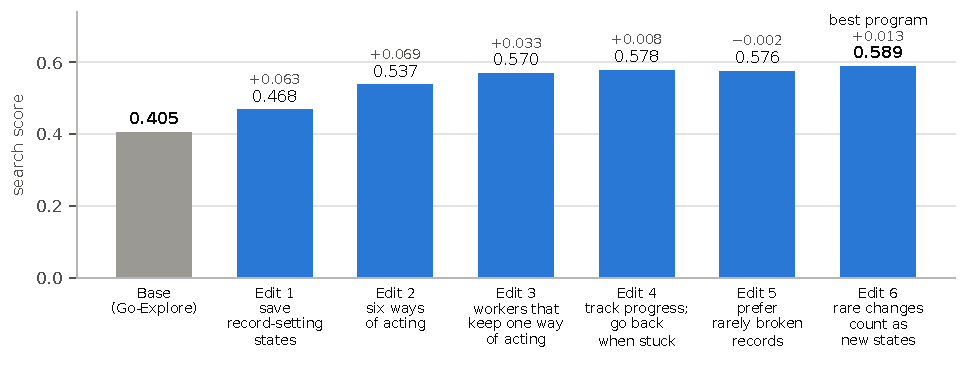
\includegraphics[width=\linewidth]{figs/fig_evolution.pdf}
\caption{\textbf{How the search reached the best program.} The best program is six edits away from the base program.
Each bar is the search score after one edit, labelled with the idea that edit added and the change in score. The other
$30$ programs the search wrote did not lead to the best one and are not shown.}
\label{fig:evo}
\end{figure}
The project had two loops. The inner loop was the search, where an LLM writes a program, then the program is scored, and the highest-scoring programs become the starting points for the next round. Fig.~\ref{fig:evo} shows how it reached the best program. The path from the base program took six edits, three by Opus and three by Sonnet. The first added record-setting states, the second added the six ways of acting, and the fourth added progress tracking. Most of the gain came from the first three edits. The outer loop was a conversation between us and the driver agent. The agent ran experiments and
reported what it found, and we decided what to do next. 

The whole project took about two weeks, and the order of events matters for how the results should be read. The search reported in this paper was started only after the evaluation bug described in Section~\ref{sec:verify} had been fixed. When it ended, its best program was saved and never edited again, and only then was it run on the four unseen games. PPO was tuned and re-run last.

\subsection{Human Interventions}
\label{sec:human}
Our involvement was steering, not execution. We checked in about twice a day to confirm the direction and to hand out
new tasks. We repeatedly asked the agent to double-check its results, its methods, and the way it framed them, and we
ran several critical reviews of its work. The evaluation bug described in Section~\ref{sec:verify} was found after we
told the agent that reporting correct results was its top priority.

Two kinds of correction came up again and again. After a critical review, the agent tended to overcorrect and play down
findings that were actually sound, and we had to push back. The agent also sometimes locked onto claims that were not
useful, so we changed the framing of the paper more than once. The biggest change came on September 2, when we moved
the paper's focus from the evaluation bug to the comparison with PPO.

The main result also depended on one specific instruction from us. Left alone, the agent kept refining a single
strategy. The search on a mix of games, which produced the program we report, exists because we told the agent to
explore other options and to write them up as separate proposals.

\subsection{Verification}
\label{sec:verify}
The first strong result of this project was wrong, and how we found out is the most useful thing we learned. The first
search produced a program that appeared to find $72\%$ of the planted bugs. The cause was a bug in the harness. When
several workers tried to save a state into the same slot at the same moment, the harness could store a mixture of their
states. Such a mixture is not a state the game can actually be in, and some of these impossible states triggered our
bug checks directly. The program's own code was fine. The search had simply favoured programs that happened to save
into the same slots often.

This result had passed every check we had at the time: a search score, both held-out sets (new levels and a new type of bug), four comparisons
against other designs, and a code review by an LLM. It failed only when we replayed detections from the start of the level. In one
scan with this program, only $12$ of $86$ detections happened again. Once the harness was fixed, the program's score on
the same setup fell from $0.578$ to $0.468$.

After this, the agent changed the harness so that only one worker can save into a slot at each step. We discarded every
search we had run and every evaluation of a program that reloads states. Replaying each detection became a permanent
part of the Kinetix evaluation, alongside a fixed set of evaluation rules, the levels and the type of bug that are kept
out of every search, and a check that removes planted bugs which no tester could ever trigger.

The replay check (Section~\ref{sec:kinetix}) does not cover every result in this paper. It covers Kinetix, which means
the scores used during the search and Table~\ref{tab:kinetix}. It does not cover the games in Fig.~\ref{fig:main},
because we did not build it for them. Those results depend on the harness bug having been fixed before they were run. It helps that PPO, random play, and action-repeat never save or reload
states, so the bug could not have affected them.

A related question is how unseen the four test games really were. They were never used to score any program during the
search, and the program was saved and frozen before it was run on them. But they were not hidden from the project.
The code that connects the grid mazes to our harness was written before the search began, and the code for Breakout
and Sokoban, including the choice of targets, was written after we had seen the program's first results on the mazes.
Several other programs were also run on these games, and we report this one because it did best. The extra levels in
Section~\ref{sec:result} are the only check that this choice could not have influenced.

Checking was shared between us and the agent. The agent wrote the replay check and ran the audits, and we did not read
the harness line by line.
We checked results by asking the agent to derive them again independently, by comparing tables that were regenerated
from the logs, and by reading the agent's running log of the project. For this version of the paper, every number in
Fig.~\ref{fig:main} and Appendix~\ref{app:perseed} was recomputed from the raw result files by a single script.

\subsection{Cost and Significance}
\label{sec:significance}
The search that produced our program cost \$$19.42$ in API calls. Scoring one program took about $15$ minutes on one GPU
and about $52$ million game steps, so the whole search used about $9$ GPU-hours and $1.9$ billion game steps. All $22$
searches we ran during the project cost about \$$270$ in API calls together. We did not keep track of the total GPU
time for the project or of the cost of the driver agent.

These numbers matter for the claim that a written tester is cheaper. For a single target, the program needs
$131{,}072$ game steps and no training, while PPO needs $4$ to $16$ times as many steps to do equally well. That is a
real saving each time the program is used. It does not make this paper's experiments cheaper overall. The one-time
search used as many game steps as about $900$ PPO runs at $16$ times the steps, and our whole comparison consists of
$240$ runs. Writing the tester only pays off if the same program is reused on many more levels or games than we tested.

If the program keeps working on other games, the practical benefit is that a small studio could test its game without
building an RL training pipeline. So far we have shown this only on small research games.

\subsection{Interpretability}
\label{sec:interp}
The output of the search is a program that a person can read. ShinkaEvolve keeps every program it produced, together
with the program it was derived from, its score, and the model that wrote it. All tables and figures are produced by
scripts from the logged results.

\subsection{Limitations}
\label{sec:limits}
The most important limitation is the games themselves. We tested only on very simple ones: small grid mazes, a
miniature Breakout, Sokoban puzzles, and a 2D physics sandbox. None of them is a commercial game, and we do not know
whether the program would work on a game with 3D worlds, long levels, or complex rules.

The comparison with PPO also has limits. It holds only when both methods get the same number of steps, and PPO catches
up with $4$ to $16$ times as many. The program can save and reload game states, and PPO was not given a way to use
that. Each game has only $6$ to $18$ targets, so the intervals are wide, and the PPO version for each game was chosen
on the same runs that we report.

Our main experiments measure exploration, not bug finding. Where we did measure bug finding, the gain was small, and
simple action-repeat was a close competitor. The main experiments were not covered by the replay check. We did not test
which parts of the program matter. Finally, the program we report stalls on the full-size Kinetix benchmark, and we do
not know why.

% ############################################################################
% ####  PART 3  ####  Reflections / broader impact
% ############################################################################
\section{Broader Impact}
The impacts of this project for game development should generally be positive. The goal was to make autonomous testing more
accessible, and with the widespread use of large language models in the current world, we believe many people can adopt and
utilize this work. Though additional work would be necessary to have it work on complex games.

Throughout the process of this autonomous loop, we found that we needed to intervene quite often. The agent had misreported
its correctness at times. At one point, the harness it wrote was broken, which inflated its score. It required finding
inconsistencies in results in order to find the leak. It is interesting to think about why it took a while. Maybe it was a
hard problem. It is also possible that an agent asked to improve a score looks less carefully at results that are already
good, though this one case cannot establish that. What we can say is that the bug was found only after the agent was told
that its top priority was to report absolutely concrete and correct findings. When doing autonomous research, if your metric
for success is something like accuracy, it is integral to build checks to ensure the results are correct, and those checks
should run the system rather than read its code.

The agent would also consistently overcorrect. If we mentioned that the direction seemed a bit vague, it would tunnel
vision immediately. If we ran an adversarial review and nitpicked at its work, then it would overcorrect. A theory we have
is that large language models tend to over-exaggerate most things, because users enjoy this, and so it takes criticism and
overcorrects to it in the same over-exaggeratory manner.

It is clear that autonomous research requires a strong research direction, with a strong harness to keep it there. It needs
something which is able to find the nuance between correcting to a director's opinion and fulfilling the research vision. It
is unclear if autonomous research can come up with its own grander ideas, as it seemed that throughout this project, we
needed to provide it with its next steps quite often. An example of lack of creativity is its continuous refining of the
same strategy rather than doing research into possibly better architectures. The current finding was only possible due to
telling the model to explore and draft up separate proposals.

Autonomous research sits in a strange place. It calls for a shift in how people approach research. Previously, you needed to
be an expert in a field just to take a step in that direction. Now, especially in software with coding agents, the
expertise you need has moved. You need less of it to implement an idea, and more of it to judge whether a result is real,
as our own harness bug showed. You steer the wheel of a (seemingly) all-knowing ship that will complete the tasks
you specify. As we spoke about in the last paragraph, this ship seems to lack much creativity and direction, and so
researchers are absolutely still necessary. But it is extremely exciting. Autonomous coding agents can contribute a
thousandfold more to open source projects and research. People who have good ideas and interesting perspectives but were
not well versed in a niche can contribute. The goal of research seems to be to advance science, after all.

Two questions from this project seem worth discussing. Who should build and check the evaluator when the same agent also
writes the candidates and the summaries? And how do you keep a test set held out while you keep redirecting the project in
response to results? We think withdrawn claims, like the first result of this project, should be reported as a matter of
routine.

% ############################################################################
\clearpage
\bibliographystyle{plainnat}
\bibliography{refs}

\appendix

\section{The evolved program}
\label{app:program}
The program is one JAX file of about $280$ lines with four functions. Below, $z$ is the feature vector rescaled to
$[-1,1]$ per entry using the running minimum and maximum over all workers. $K$ is the number of archive slots and $B$ the
number of workers. All constants were set by the search.

\textbf{State kept while running.} Per feature: running minimum and maximum; decayed counts of upward and downward moves
(decay $0.995$); a decayed rate of how often the feature changes at all (decay $0.999$); a decayed rate of how often its
record is broken. Per behaviour: decayed reward and decayed step count (decay $0.99$). Per worker: current behaviour and
its remaining segment length, and a count of consecutive steps without movement.

\textbf{Derived quantities.}
\begin{itemize}
\item \emph{Ratchet weight} of a feature: $0$ if fewer than $80\%$ of its moves are upward, rising linearly to $1$ at
$100\%$.
\item \emph{Rarity} of a feature: close to $1$ if it changes on few steps, close to $0$ if it changes on most steps
(trusted after $30$ samples).
\item \emph{Depth} of a state: the weighted mean of its rescaled features, with weight $\max(\text{ratchet},\,
0.5\cdot\text{rarity})$. It is $0$ if no feature qualifies.
\item \emph{Cell} of a state: a $14$-bit random-projection hash of eight rescaled entries rounded to $0.4$, combined (XOR)
with an exact $5$-level quantisation of every feature whose rarity exceeds $0.3$.
\end{itemize}

\textbf{How saved states are managed.} The program does not keep a list of saved states sorted by usefulness. It has a
fixed number of slots ($128$ in our main experiments). Which slot a state goes into is decided when it is saved, and how
useful each saved state is gets recomputed from scratch every time a worker restores. A slot is reused when something
better for that slot arrives, as described under \texttt{archive}.

\textbf{\texttt{restore}} (for each worker, each step).
\begin{enumerate}
\item Trigger with probability $0.03 + 0.12\cdot(\text{elapsed fraction of the episode})$, or if the worker has not moved
for more than $40$ steps. One worker in five never restores.
\item Score every saved state: $+1$ if it is a frontier slot, plus $0.6$ times the rarity of the record it holds; minus
$0.5\cdot\log(1+\text{visits})$; plus $0.5$ times its rescaled entry $4$ (speed on Kinetix, the progress scalar on other
engines); plus $w\cdot\text{depth}$, where $w=2.5$ for every
third worker and $1$ for the rest.
\item Add Gumbel noise and jump to the highest-scoring state. This amounts to picking a saved state at random, with
higher-scoring states more likely. A restored worker starts a new behaviour segment.
\end{enumerate}

\textbf{\texttt{act}} (for each worker, each step).
\begin{enumerate}
\item If the segment has ended, draw a behaviour from the bandit: a softmax (sharpness $3$) over each behaviour's recent
reward per step, mixed with a $25\%$ uniform floor. One worker in four keeps a fixed behaviour for the whole run. Draw a
segment length up to a per-behaviour maximum of $6$, $14$, $45$, $48$, $80$, or $64$ steps.
\item Behaviours: (a) a fresh random action each step; (b) one random action repeated; (c) the first or last action held;
(d) a sweep through all actions, each held for $1$ to $8$ steps; (e) switch between two actions according to the sign of
a sparse random projection of $z$; (f) the action that maximises a sparse random linear function of $z$ plus noise.
\item Update the worker's stuck counter from the change in $z$.
\end{enumerate}

\textbf{\texttt{archive}} (for each worker, each step).
\begin{enumerate}
\item \emph{Frontier.} If the worker's state exceeds the running maximum or minimum of any feature by more than $5\%$ of
that feature's range, save it in the frontier slot for that feature and direction ($35\%$ of slots), replacing the
previous record. Elapsed time is excluded. When there are more features than frontier slots, several features share a
slot, and the most recent record wins.
\item \emph{Coverage.} Otherwise compute the state's cell. If the cell is empty, save the state in the next coverage
slot. Coverage slots are filled in order, and once all are full the oldest is overwritten. If the cell is occupied,
replace the occupant only if entry $4$ plus $0.5\cdot$depth is higher by more than $0.05$.
\item \emph{Bandit reward} for the worker's current behaviour: $1$ for a new record, scaled up when that record is rarely
broken; $0.25$ for a new cell; the gain in depth this step; and the rarity of any rare feature that moved.
\item Update all running statistics.
\end{enumerate}

\section{Protocol details}
\label{app:protocol}
\textbf{Feature vector.} Entries $0$ to $10$ have a fixed meaning on every engine: position ($2$), velocity ($2$), a
progress or speed scalar ($1$), agent position ($2$), distance to the target if the engine exposes one or a constant
otherwise ($1$), elapsed time fraction ($1$), target position or a constant ($2$). The remaining entries are
engine-specific. On MiniGrid the progress scalar is whether an object is carried and the tail holds direction and grid
contents. On Sokoban it is the number of boxes on goals. On Breakout it is the number of bricks cleared. On DeepSea it is
depth. Positions are scaled to $[0,5]$ on every engine. These adapters were written by the driver agent. PPO receives the
same vector.

\textbf{Testers.} $64$ workers, $2048$ steps, $128$ archive slots, five seeds ($32$ workers and three seeds on Craftax). On
Craftax the testers were run on $40$ targets and PPO on $48$; we report the $32$ that both were run on.
All workers of one run share one level.

\textbf{Go-Explore.} A $12$-bit random-projection hash of feature entries $(0,1,2,3,5,6,9,10)$ rounded to $0.5$. One state
is stored per new cell. Each worker restores with probability $0.05$ per step to a slot sampled with weight
$1/\sqrt{1+\text{visits}}$. Actions are random and held for $1$ to $12$ steps. No constants were tuned. The cell does not
include the progress scalar, so on DoorKey two states at the same position with and without the key share a cell.

\textbf{PPO.} Policy and value are separate MLPs with two hidden layers of $128$ units. Discount $0.99$, GAE $\lambda$
$0.95$, clip $0.2$, value coefficient $0.5$, gradient clip $0.5$, four epochs, four minibatches, Adam. Default setting:
learning rate $3\cdot10^{-4}$, entropy coefficient $0.01$. Tuned setting: $10^{-4}$ and $0.2$. Intrinsic objectives use
the intrinsic reward only; the task objective uses the task reward only. Budgets: $64$ environments, $64$-step rollouts,
and $32$, $128$, or $512$ updates for $1\times$, $4\times$, $16\times$. Selected configurations at $1\times$: count bonus
(DoorKey, FourRooms), task reward (Breakout), proximity-curiosity (Sokoban), all with the tuned setting. At $4\times$ and
$16\times$ the candidates were count, ICM, and proximity-curiosity with the tuned setting and three seeds.

\textbf{Kinetix protocol.} $128$ workers, $2048$ steps, $256$ slots, evaluation seeds $100$ to $104$; fitness seeds $0$
to $2$ at $128$ workers and $1024$ steps. Excluded instances: $8$ of $127$ on search levels, $1$ of $59$ on held-out
levels, $0$ of $148$ in the held-out class. PPO rows use three training seeds.

\section{Per-seed results and extra levels}
\label{app:perseed}
\begin{table}[h]\centering\small
\caption{Fraction of targets reached per seed at equal budget (five seeds each).}
\label{tab:perseed}
\setlength{\tabcolsep}{4pt}
\begin{tabular}{@{}lllll@{}}\toprule
 & DoorKey & FourRooms & Breakout & Sokoban \\ \midrule
Evolved program & 1, 1, 1, 1, 1 & .67, .83, 1, 1, .83 & 1, 1, 1, 1, 1 & .83, .72, .83, .83, .72 \\
PPO, tuned & .83, .83, .83, .83, .83 & .50, .17, .67, .50, .67 & .44, .39, .50, .44, .33 & .56, .56, .33, .28, .33 \\
Random & .83, .83, .83, .50, .83 & .33, .33, .17, .17, .33 & .33, .33, .33, .33, .33 & .78, .67, .56, .67, .61 \\
Action-repeat & .33, .33, .17, .33, .50 & .33, .33, .33, .50, .50 & .33, .33, .33, .33, .33 & .61, .56, .56, .56, .50 \\
Go-Explore & .17, .17, .17, 0, 0 & .33, .50, .33, .33, .50 & .33, .33, .33, .33, .33 & .50, .56, .44, .56, .50 \\ \bottomrule
\end{tabular}
\end{table}
On Breakout, random, action-repeat, and Go-Explore reach exactly the six targets with the lowest threshold (three bricks)
on every seed, which is why they sit at $0.33$.

\begin{table}[h]\centering\small
\caption{Extra levels that were not used when choosing which program to report (mean over five seeds). $n$ is the number
of targets.}
\label{tab:heldout}
\begin{tabular}{@{}lcccc@{}}\toprule
 & DoorKey ($n{=}2$) & FourRooms ($n{=}2$) & Breakout ($n{=}6$) & Sokoban ($n{=}6$) \\ \midrule
Evolved program & 1.00 & 0.20 & 1.00 & 0.80 \\
PPO, tuned & 0.80 & 0.40 & 0.40 & 0.37 \\
Random & 1.00 & 0.20 & 0.33 & 0.70 \\
Action-repeat & 0.00 & 0.50 & 0.33 & 0.47 \\
Go-Explore & 0.00 & 0.40 & 0.33 & 0.40 \\ \bottomrule
\end{tabular}
\end{table}

\section{Search details}
\label{app:search}
\textbf{Task description given to the proposal models} (abridged; the interface signatures and coding rules are
omitted). ``You are improving a game-testing program for 2D physics puzzle games (Kinetix, JAX). A batch of B workers
explores one level; the harness keeps K archive slots of saved states. Your program defines four pure-JAX hooks [\ldots]
The fitness is how quickly the workers reach states that expose planted defects (leaving the arena, passing through a
solid, winning via an unintended goal, runaway physics, touching a disarmed hazard) across many levels, measured as
1 - steps\_to\_first\_witness/budget, averaged. A held-out defect class and held-out levels are NOT in the fitness; programs
that overfit the visible classes will not transfer, so prefer general exploration strategies (systematic coverage of
position/velocity space, reaching extreme states, high-energy interactions, varied action patterns, archive diversity).
[\ldots] Only modify code between the EVOLVE-BLOCK markers.''

\textbf{How programs were scored in the search.} The score (called fitness in ShinkaEvolve) is a weighted mean of $1-\min(\text{first hit},\text{budget})/\text{budget}$ over
targets and seeds $\{0,1,2\}$: Kinetix planted defects ($103$ reachable search targets, $128$ workers, $1024$ steps,
weight $1.0$); Craftax ($32$ workers, $2048$ steps, weight $1.0$); MountainCar, Acrobot, and DeepSea-8 ($64$ workers,
$512$ steps, weights $0.34$, $0.33$, $0.33$).

\textbf{Search settings.} ShinkaEvolve kept two separate pools of programs (islands), each holding up to $30$ programs,
and copied programs between them every $10$ rounds (migration rate $0.1$). The program to improve was chosen with
ShinkaEvolve's ``weighted'' parent selection, and the model was also shown four other programs for inspiration, two
from the pool and two of the highest-scoring ones. Two programs were written and two were scored at a time. The search
was set to stop after $40$ rounds or \$$40$ of API cost.

\textbf{Edits.} Of the $36$ scored programs, about $20$ were diffs, $9$ full rewrites, and $6$ crossovers. The reported
program is six edits away from the base program (Fig.~\ref{fig:evo}): three by Opus and three by Sonnet, of which
four were diffs, one a full rewrite, and one a crossover.

\section{Reproducibility Statement}
The main result is the equal-budget comparison in Fig.~\ref{fig:main}; the second is the Kinetix study in
Table~\ref{tab:kinetix}. Reproducing them requires the evolved program (one JAX file), the task splits, the baselines in
the same harness, and for Kinetix the frozen protocol and the replay verifier. Sections~\ref{sec:setup}
to~\ref{sec:protocol} and Appendices~\ref{app:program} and~\ref{app:protocol} give the interface, budgets, targets, seeds,
selection rule, and hyperparameters. Code, splits, logs, every candidate program, and the scripts that produce the figures
and tables are available at \url{https://github.com/andyye132/AutoDEV}.

\section{Disclosure Statement}

\paragraph{Agent(s) / model(s) used.}
The tester programs were written by an autonomous ShinkaEvolve loop using \texttt{claude-sonnet-5} and
\texttt{claude-opus-5} as proposal models. The project was driven by an interactive Claude agent (\texttt{claude-fable-5}),
which built the harness, benchmark, and baselines, ran the experiments and analysis, and drafted Part~1. Part~2, Part~3,
and this statement were written by the human author. For the camera-ready version, the paper was restructured and its
numbers were recomputed with the help of an interactive Claude agent, in response to the reviews, and the human author
reviewed the result.

\begin{itemize}
  \item[$\boxtimes$] A human author has curated this work and verified every claim,
    figure, methodology detail, and reference.
  \item[$\boxtimes$] A human author takes full accountability for the submission as
    a human-authored, human-verified artifact.
\end{itemize}

\section*{NeurIPS Paper Checklist}




\begin{enumerate}

\item {\bf Claims}
    \item[] Question: Do the main claims made in the abstract and introduction accurately reflect the paper's contributions and scope?
    \item[] Answer: \answerYes{} % Replace by \answerYes{}, \answerNo{}, or \answerNA{}.
    \item[] Justification: The abstract and introduction state the main claim (target reaching at an equal step budget on four tasks outside the search) and its limits: the program needs save and restore access, ties trivial baselines on two tasks, shows no advantage on Craftax, is matched by PPO at $4$--$16\times$ the interaction, and bug detection is measured only on Kinetix. These match Section~\ref{sec:result}, Section~\ref{sec:kinetix}, and Section~\ref{sec:limits}.
    \item[] Guidelines:
    \begin{itemize}
        \item The answer \answerNA{} means that the abstract and introduction do not include the claims made in the paper.
        \item The abstract and/or introduction should clearly state the claims made, including the contributions made in the paper and important assumptions and limitations. A \answerNo{} or \answerNA{} answer to this question will not be perceived well by the reviewers. 
        \item The claims made should match theoretical and experimental results, and reflect how much the results can be expected to generalize to other settings. 
        \item It is fine to include aspirational goals as motivation as long as it is clear that these goals are not attained by the paper. 
    \end{itemize}

\item {\bf Limitations}
    \item[] Question: Does the paper discuss the limitations of the work performed by the authors?
    \item[] Answer: \answerYes{} % Replace by \answerYes{}, \answerNo{}, or \answerNA{}.
    \item[] Justification: Section~\ref{sec:limits} lists the limits (equal budget only, simulator access, target reaching versus bug detection, scope of replay verification, small task sizes, PPO selection, no ablations, simple 2D environments), and Section~\ref{sec:result} reports the tasks where the program does not win.
    \item[] Guidelines:
    \begin{itemize}
        \item The answer \answerNA{} means that the paper has no limitation while the answer \answerNo{} means that the paper has limitations, but those are not discussed in the paper. 
        \item The authors are encouraged to create a separate ``Limitations'' section in their paper.
        \item The paper should point out any strong assumptions and how robust the results are to violations of these assumptions (e.g., independence assumptions, noiseless settings, model well-specification, asymptotic approximations only holding locally). The authors should reflect on how these assumptions might be violated in practice and what the implications would be.
        \item The authors should reflect on the scope of the claims made, e.g., if the approach was only tested on a few datasets or with a few runs. In general, empirical results often depend on implicit assumptions, which should be articulated.
        \item The authors should reflect on the factors that influence the performance of the approach. For example, a facial recognition algorithm may perform poorly when image resolution is low or images are taken in low lighting. Or a speech-to-text system might not be used reliably to provide closed captions for online lectures because it fails to handle technical jargon.
        \item The authors should discuss the computational efficiency of the proposed algorithms and how they scale with dataset size.
        \item If applicable, the authors should discuss possible limitations of their approach to address problems of privacy and fairness.
        \item While the authors might fear that complete honesty about limitations might be used by reviewers as grounds for rejection, a worse outcome might be that reviewers discover limitations that aren't acknowledged in the paper. The authors should use their best judgment and recognize that individual actions in favor of transparency play an important role in developing norms that preserve the integrity of the community. Reviewers will be specifically instructed to not penalize honesty concerning limitations.
    \end{itemize}

\item {\bf Theory assumptions and proofs}
    \item[] Question: For each theoretical result, does the paper provide the full set of assumptions and a complete (and correct) proof?
    \item[] Answer: \answerNA{} % Replace by \answerYes{}, \answerNo{}, or \answerNA{}.
    \item[] Justification: The paper is empirical and makes no theoretical claims; it contains no theorems or proofs.
    \item[] Guidelines:
    \begin{itemize}
        \item The answer \answerNA{} means that the paper does not include theoretical results. 
        \item All the theorems, formulas, and proofs in the paper should be numbered and cross-referenced.
        \item All assumptions should be clearly stated or referenced in the statement of any theorems.
        \item The proofs can either appear in the main paper or the supplemental material, but if they appear in the supplemental material, the authors are encouraged to provide a short proof sketch to provide intuition. 
        \item Inversely, any informal proof provided in the core of the paper should be complemented by formal proofs provided in appendix or supplemental material.
        \item Theorems and Lemmas that the proof relies upon should be properly referenced. 
    \end{itemize}

    \item {\bf Experimental result reproducibility}
    \item[] Question: Does the paper fully disclose all the information needed to reproduce the main experimental results of the paper to the extent that it affects the main claims and/or conclusions of the paper (regardless of whether the code and data are provided or not)?
    \item[] Answer: \answerYes{} % Replace by \answerYes{}, \answerNo{}, or \answerNA{}.
    \item[] Justification: Sections~\ref{sec:setup}--\ref{sec:protocol} and Appendices~\ref{app:program}--\ref{app:search} give the tester interface, pseudocode and constants of the evolved program, budgets, targets, seeds, the PPO selection rule, baseline details, and the search configuration; code and logs are released.
    \item[] Guidelines:
    \begin{itemize}
        \item The answer \answerNA{} means that the paper does not include experiments.
        \item If the paper includes experiments, a \answerNo{} answer to this question will not be perceived well by the reviewers: Making the paper reproducible is important, regardless of whether the code and data are provided or not.
        \item If the contribution is a dataset and\slash or model, the authors should describe the steps taken to make their results reproducible or verifiable. 
        \item Depending on the contribution, reproducibility can be accomplished in various ways. For example, if the contribution is a novel architecture, describing the architecture fully might suffice, or if the contribution is a specific model and empirical evaluation, it may be necessary to either make it possible for others to replicate the model with the same dataset, or provide access to the model. In general. releasing code and data is often one good way to accomplish this, but reproducibility can also be provided via detailed instructions for how to replicate the results, access to a hosted model (e.g., in the case of a large language model), releasing of a model checkpoint, or other means that are appropriate to the research performed.
        \item While NeurIPS does not require releasing code, the conference does require all submissions to provide some reasonable avenue for reproducibility, which may depend on the nature of the contribution. For example
        \begin{enumerate}
            \item If the contribution is primarily a new algorithm, the paper should make it clear how to reproduce that algorithm.
            \item If the contribution is primarily a new model architecture, the paper should describe the architecture clearly and fully.
            \item If the contribution is a new model (e.g., a large language model), then there should either be a way to access this model for reproducing the results or a way to reproduce the model (e.g., with an open-source dataset or instructions for how to construct the dataset).
            \item We recognize that reproducibility may be tricky in some cases, in which case authors are welcome to describe the particular way they provide for reproducibility. In the case of closed-source models, it may be that access to the model is limited in some way (e.g., to registered users), but it should be possible for other researchers to have some path to reproducing or verifying the results.
        \end{enumerate}
    \end{itemize}


\item {\bf Open access to data and code}
    \item[] Question: Does the paper provide open access to the data and code, with sufficient instructions to faithfully reproduce the main experimental results, as described in supplemental material?
    \item[] Answer: \answerYes{} % Replace by \answerYes{}, \answerNo{}, or \answerNA{}.
    \item[] Justification: Code, the benchmark, task splits, logs, every candidate program, and the scripts that regenerate the figures and tables are released at the URL in the Reproducibility Statement.
    \item[] Guidelines:
    \begin{itemize}
        \item The answer \answerNA{} means that paper does not include experiments requiring code.
        \item Please see the NeurIPS code and data submission guidelines (\url{https://neurips.cc/public/guides/CodeSubmissionPolicy}) for more details.
        \item While we encourage the release of code and data, we understand that this might not be possible, so \answerNo{} is an acceptable answer. Papers cannot be rejected simply for not including code, unless this is central to the contribution (e.g., for a new open-source benchmark).
        \item The instructions should contain the exact command and environment needed to run to reproduce the results. See the NeurIPS code and data submission guidelines (\url{https://neurips.cc/public/guides/CodeSubmissionPolicy}) for more details.
        \item The authors should provide instructions on data access and preparation, including how to access the raw data, preprocessed data, intermediate data, and generated data, etc.
        \item The authors should provide scripts to reproduce all experimental results for the new proposed method and baselines. If only a subset of experiments are reproducible, they should state which ones are omitted from the script and why.
        \item At submission time, to preserve anonymity, the authors should release anonymized versions (if applicable).
        \item Providing as much information as possible in supplemental material (appended to the paper) is recommended, but including URLs to data and code is permitted.
    \end{itemize}


\item {\bf Experimental setting/details}
    \item[] Question: Does the paper specify all the training and test details (e.g., data splits, hyperparameters, how they were chosen, type of optimizer) necessary to understand the results?
    \item[] Answer: \answerYes{} % Replace by \answerYes{}, \answerNo{}, or \answerNA{}.
    \item[] Justification: Section~\ref{sec:setup}, Section~\ref{sec:protocol}, Table~\ref{tab:protocol}, and Appendix~\ref{app:protocol} give the step budgets, target definitions and counts, seeds, PPO objectives and hyperparameters, how the PPO configuration was selected, and the baseline settings.
    \item[] Guidelines:
    \begin{itemize}
        \item The answer \answerNA{} means that the paper does not include experiments.
        \item The experimental setting should be presented in the core of the paper to a level of detail that is necessary to appreciate the results and make sense of them.
        \item The full details can be provided either with the code, in appendix, or as supplemental material.
    \end{itemize}

\item {\bf Experiment statistical significance}
    \item[] Question: Does the paper report error bars suitably and correctly defined or other appropriate information about the statistical significance of the experiments?
    \item[] Answer: \answerYes{} % Replace by \answerYes{}, \answerNo{}, or \answerNA{}.
    \item[] Justification: Figure~\ref{fig:main} shows $95\%$ bootstrap intervals that resample targets and seeds, Section~\ref{sec:result} gives paired intervals against PPO, and Appendix~\ref{app:perseed} lists per-seed values. Table~\ref{tab:kinetix} reports means over five seeds.
    \item[] Guidelines:
    \begin{itemize}
        \item The answer \answerNA{} means that the paper does not include experiments.
        \item The authors should answer \answerYes{} if the results are accompanied by error bars, confidence intervals, or statistical significance tests, at least for the experiments that support the main claims of the paper.
        \item The factors of variability that the error bars are capturing should be clearly stated (for example, train/test split, initialization, random drawing of some parameter, or overall run with given experimental conditions).
        \item The method for calculating the error bars should be explained (closed form formula, call to a library function, bootstrap, etc.)
        \item The assumptions made should be given (e.g., Normally distributed errors).
        \item It should be clear whether the error bar is the standard deviation or the standard error of the mean.
        \item It is OK to report 1-sigma error bars, but one should state it. The authors should preferably report a 2-sigma error bar than state that they have a 96\% CI, if the hypothesis of Normality of errors is not verified.
        \item For asymmetric distributions, the authors should be careful not to show in tables or figures symmetric error bars that would yield results that are out of range (e.g., negative error rates).
        \item If error bars are reported in tables or plots, the authors should explain in the text how they were calculated and reference the corresponding figures or tables in the text.
    \end{itemize}

\item {\bf Experiments compute resources}
    \item[] Question: For each experiment, does the paper provide sufficient information on the computer resources (type of compute workers, memory, time of execution) needed to reproduce the experiments?
    \item[] Answer: \answerYes{} % Replace by \answerYes{}, \answerNo{}, or \answerNA{}.
    \item[] Justification: Section~\ref{sec:tools} reports the hardware and Section~\ref{sec:significance} reports the search cost (API dollars, GPU-hours, simulator steps). Total GPU-hours for the whole project and the cost of the driver agent were not recorded, which we state.
    \item[] Guidelines:
    \begin{itemize}
        \item The answer \answerNA{} means that the paper does not include experiments.
        \item The paper should indicate the type of compute workers CPU or GPU, internal cluster, or cloud provider, including relevant memory and storage.
        \item The paper should provide the amount of compute required for each of the individual experimental runs as well as estimate the total compute. 
        \item The paper should disclose whether the full research project required more compute than the experiments reported in the paper (e.g., preliminary or failed experiments that didn't make it into the paper). 
    \end{itemize}
    
\item {\bf Code of ethics}
    \item[] Question: Does the research conducted in the paper conform, in every respect, with the NeurIPS Code of Ethics \url{https://neurips.cc/public/EthicsGuidelines}?
    \item[] Answer: \answerYes{} % Replace by \answerYes{}, \answerNo{}, or \answerNA{}.
    \item[] Justification: The research conforms to the NeurIPS Code of Ethics. It involves no human subjects, no personal or sensitive data, and no deployed system with foreseeable harm.
    \item[] Guidelines:
    \begin{itemize}
        \item The answer \answerNA{} means that the authors have not reviewed the NeurIPS Code of Ethics.
        \item If the authors answer \answerNo, they should explain the special circumstances that require a deviation from the Code of Ethics.
        \item The authors should make sure to preserve anonymity (e.g., if there is a special consideration due to laws or regulations in their jurisdiction).
    \end{itemize}


\item {\bf Broader impacts}
    \item[] Question: Does the paper discuss both potential positive societal impacts and negative societal impacts of the work performed?
    \item[] Answer: \answerYes{} % Replace by \answerYes{}, \answerNo{}, or \answerNA{}.
    \item[] Justification: The Broader Impact section discusses the positive impact of cheaper, more accessible game testing and reflects on the reliability and oversight of autonomous research loops.
    \item[] Guidelines:
    \begin{itemize}
        \item The answer \answerNA{} means that there is no societal impact of the work performed.
        \item If the authors answer \answerNA{} or \answerNo, they should explain why their work has no societal impact or why the paper does not address societal impact.
        \item Examples of negative societal impacts include potential malicious or unintended uses (e.g., disinformation, generating fake profiles, surveillance), fairness considerations (e.g., deployment of technologies that could make decisions that unfairly impact specific groups), privacy considerations, and security considerations.
        \item The conference expects that many papers will be foundational research and not tied to particular applications, let alone deployments. However, if there is a direct path to any negative applications, the authors should point it out. For example, it is legitimate to point out that an improvement in the quality of generative models could be used to generate Deepfakes for disinformation. On the other hand, it is not needed to point out that a generic algorithm for optimizing neural networks could enable people to train models that generate Deepfakes faster.
        \item The authors should consider possible harms that could arise when the technology is being used as intended and functioning correctly, harms that could arise when the technology is being used as intended but gives incorrect results, and harms following from (intentional or unintentional) misuse of the technology.
        \item If there are negative societal impacts, the authors could also discuss possible mitigation strategies (e.g., gated release of models, providing defenses in addition to attacks, mechanisms for monitoring misuse, mechanisms to monitor how a system learns from feedback over time, improving the efficiency and accessibility of ML).
    \end{itemize}
    
\item {\bf Safeguards}
    \item[] Question: Does the paper describe safeguards that have been put in place for responsible release of data or models that have a high risk for misuse (e.g., pre-trained language models, image generators, or scraped datasets)?
    \item[] Answer: \answerNA{} % Replace by \answerYes{}, \answerNo{}, or \answerNA{}.
    \item[] Justification: The paper releases no high-risk models or data; the artifacts are game-testing exploration programs and a physics-simulation defect benchmark with no foreseeable misuse requiring safeguards.
    \item[] Guidelines:
    \begin{itemize}
        \item The answer \answerNA{} means that the paper poses no such risks.
        \item Released models that have a high risk for misuse or dual-use should be released with necessary safeguards to allow for controlled use of the model, for example by requiring that users adhere to usage guidelines or restrictions to access the model or implementing safety filters. 
        \item Datasets that have been scraped from the Internet could pose safety risks. The authors should describe how they avoided releasing unsafe images.
        \item We recognize that providing effective safeguards is challenging, and many papers do not require this, but we encourage authors to take this into account and make a best faith effort.
    \end{itemize}

\item {\bf Licenses for existing assets}
    \item[] Question: Are the creators or original owners of assets (e.g., code, data, models), used in the paper, properly credited and are the license and terms of use explicitly mentioned and properly respected?
    \item[] Answer: \answerYes{} % Replace by \answerYes{}, \answerNo{}, or \answerNA{}.
    \item[] Justification: All external assets are open-source research packages and are cited: the simulators (Kinetix, MiniGrid, MinAtar, Jumanji, Gymnax, Craftax) and the evolution framework ShinkaEvolve~\citep{shinkaevolve}, each used under its own license.
    \item[] Guidelines:
    \begin{itemize}
        \item The answer \answerNA{} means that the paper does not use existing assets.
        \item The authors should cite the original paper that produced the code package or dataset.
        \item The authors should state which version of the asset is used and, if possible, include a URL.
        \item The name of the license (e.g., CC-BY 4.0) should be included for each asset.
        \item For scraped data from a particular source (e.g., website), the copyright and terms of service of that source should be provided.
        \item If assets are released, the license, copyright information, and terms of use in the package should be provided. For popular datasets, \url{paperswithcode.com/datasets} has curated licenses for some datasets. Their licensing guide can help determine the license of a dataset.
        \item For existing datasets that are re-packaged, both the original license and the license of the derived asset (if it has changed) should be provided.
        \item If this information is not available online, the authors are encouraged to reach out to the asset's creators.
    \end{itemize}

\item {\bf New assets}
    \item[] Question: Are new assets introduced in the paper well documented and is the documentation provided alongside the assets?
    \item[] Answer: \answerYes{} % Replace by \answerYes{}, \answerNo{}, or \answerNA{}.
    \item[] Justification: The planted-defect benchmark and the tester programs are described in Section~\ref{sec:kinetix}, Section~\ref{sec:method}, and Appendix~\ref{app:program}, and are released with the code.
    \item[] Guidelines:
    \begin{itemize}
        \item The answer \answerNA{} means that the paper does not release new assets.
        \item Researchers should communicate the details of the dataset\slash code\slash model as part of their submissions via structured templates. This includes details about training, license, limitations, etc. 
        \item The paper should discuss whether and how consent was obtained from people whose asset is used.
        \item At submission time, remember to anonymize your assets (if applicable). You can either create an anonymized URL or include an anonymized zip file.
    \end{itemize}

\item {\bf Crowdsourcing and research with human subjects}
    \item[] Question: For crowdsourcing experiments and research with human subjects, does the paper include the full text of instructions given to participants and screenshots, if applicable, as well as details about compensation (if any)? 
    \item[] Answer: \answerNA{} % Replace by \answerYes{}, \answerNo{}, or \answerNA{}.
    \item[] Justification: The research does not involve crowdsourcing or human subjects.
    \item[] Guidelines:
    \begin{itemize}
        \item The answer \answerNA{} means that the paper does not involve crowdsourcing nor research with human subjects.
        \item Including this information in the supplemental material is fine, but if the main contribution of the paper involves human subjects, then as much detail as possible should be included in the main paper. 
        \item According to the NeurIPS Code of Ethics, workers involved in data collection, curation, or other labor should be paid at least the minimum wage in the country of the data collector. 
    \end{itemize}

\item {\bf Institutional review board (IRB) approvals or equivalent for research with human subjects}
    \item[] Question: Does the paper describe potential risks incurred by study participants, whether such risks were disclosed to the subjects, and whether Institutional Review Board (IRB) approvals (or an equivalent approval/review based on the requirements of your country or institution) were obtained?
    \item[] Answer: \answerNA{} % Replace by \answerYes{}, \answerNo{}, or \answerNA{}.
    \item[] Justification: The research does not involve human subjects, so IRB approval is not applicable.
    \item[] Guidelines:
    \begin{itemize}
        \item The answer \answerNA{} means that the paper does not involve crowdsourcing nor research with human subjects.
        \item Depending on the country in which research is conducted, IRB approval (or equivalent) may be required for any human subjects research. If you obtained IRB approval, you should clearly state this in the paper. 
        \item We recognize that the procedures for this may vary significantly between institutions and locations, and we expect authors to adhere to the NeurIPS Code of Ethics and the guidelines for their institution. 
        \item For initial submissions, do not include any information that would break anonymity (if applicable), such as the institution conducting the review.
    \end{itemize}

\item {\bf Declaration of LLM usage}
    \item[] Question: Does the paper describe the usage of LLMs if it is an important, original, or non-standard component of the core methods in this research? Note that if the LLM is used only for writing, editing, or formatting purposes and does \emph{not} impact the core methodology, scientific rigor, or originality of the research, declaration is not required.
    %this research? 
    \item[] Answer: \answerYes{} % Replace by \answerYes{}, \answerNo{}, or \answerNA{}.
    \item[] Justification: LLM usage is central and disclosed. Section~\ref{sec:roles}, Section~\ref{sec:agent}, and the Disclosure Statement describe the evolution loop (\texttt{claude-sonnet-5} and \texttt{claude-opus-5} as proposal models) that wrote the tester programs, and the interactive driver agent (\texttt{claude-fable-5}) that built the harness, ran the experiments, and drafted Part~1.
    \item[] Guidelines:
    \begin{itemize}
        \item The answer \answerNA{} means that the core method development in this research does not involve LLMs as any important, original, or non-standard components.
        \item Please refer to our LLM policy in the NeurIPS handbook for what should or should not be described.
    \end{itemize}

\end{enumerate}

\end{document}
